\documentclass[12pt]{article}

\title{Applying Natural Language Processing and Machine Learning techniques to aid in the diagnosis of Mild Cognitive Impairment and Early Dementia - A Systematic Review}

\author{
	Jomar Alcantara \\
	Department of Computer Science\\
	School of Engineering and Applied Sciences\\
	Aston University\\
	\texttt{alcantaj@aston.ac.uk} \\
		\AND
	Peter Sawyer \\
	Department of Computer Science\\
	School of Engineering and Applied Sciences\\
	Aston University\\
	\texttt{p.sawyer@aston.ac.uk}
		\AND
	George Vogiatzis\\
	Department of Computer Science\\
	School of Engineering and Applied Sciences\\
	Aston University \\
	\texttt{g.vogiatzis@aston.ac.uk} \\
		\AND
	Cristina Romani\\
	Department of Psychology\\
	School of Life and Health Sciences\\
	Aston University \\
	\texttt{c.romani@aston.ac.uk}
}
	
\date{\today}

\usepackage{arxiv}
\usepackage{float} % allows precise placement of tables
\usepackage[utf8]{inputenc} % allow utf-8 input
\usepackage[T1]{fontenc}    % use 8-bit T1 fonts
\usepackage{hyperref}       % hyperlinks
\usepackage{url}            % simple URL typesetting
\usepackage{booktabs}       % professional-quality tables
\usepackage{amsfonts}       % blackboard math symbols
\usepackage{nicefrac}       % compact symbols for 1/2, etc.
\usepackage{microtype}      % microtypography
\usepackage{longtable}		% for use in table in Appendix A


\begin{document}
\maketitle

\keywords{MCI \and Alzheimer's Disease \and Machine Learning \and Diagnosis} 
\bigskip
\begin{abstract}
Dementia is a growing problem which faces the world today with the total worldwide cost of dementia last year projected to be in the region of one trillion US dollars. Given the huge impact Dementia has, a lot of research has been focused on finding ways to improve the early diagnosis of dementia and Mild Cognitive Impairment. Equally, our ability to process language and find patterns of decline using the techniques of Natural Language Processing and Machine Learning has vastly increased over the recent times. This represents an opportunity to harness these techniques to find patterns in cognitive decline that could indicate the presence of the early stages of dementia.  This paper looks at body of research focused on the analysis of cognitive decline in those suspected to have dementia. Specifically,   \ldots
\end{abstract}

\section{Introduction}
Dementia has been identified as one of the fast growing difficulties facing the world. A recent report suggests that in 2015 there were 46 million people with a diagnosis of dementia and that number is expected to hit 131.5 million by 2050 \cite{Prince2015}. The report also states that the worldwide cost of dementia in 2018 is estimated to be in the region of one trillion US dollars.
\par
A lot of work has gone into trying to find ways of improving the early diagnosis of Alzheimer's Disease (AD) and Mild Cognitive Impairment (MCI) with research focused on two areas - identifying biological markers and analyzing the cognitive decline of those who are suspected to have the disease \cite{Taler2008}. As described above \cite{Prince2015}, the numbers of those suffering from AD and MCI are going to increase as the population ages and thus it is important that we utilize technology wherever possible to aid clinicians in the detection of MCI and AD. At the present time diagnosis is typically conducted at memory clinics by trained clinicians \cite{Boschi2017}. I theorize that we may be able to enable an earlier diagnosis of those with MCI and AD using samples of spontaneous speech, natural language processing (NLP) and machine learning (ML).
\par
There is a large body of research that looks at language deterioration in those suspected to have MCI or AD \cite{Taler2008, Boschi2017}. However there is conflicting evidence in these studies about which declining language factors are associated with MCI and AD \cite{Taler2008, Boschi2017}. Research therefore, should look at these features in more detail and a clarification of this currently disorganised picture should go some way to helping researchers further understand the disease and it's progression. Another area of focus for research of this nature is the process of collecting appropriate language samples. Whilst collecting samples of language is comparatively unintrusive, researchers recognise that these samples require a rich sample of language that potentially cannot be generated by tasks such as the picture description task. Therefore, it would be useful to explore whether spontaneous discourse such a semi-structured interview, has the ability to put pressure on both the cognitive and linguistic systems in the same way as traditional cognitive tests such that it might be able to distinguish between healthy controls, those with MCI and those with AD. There is some evidence to support this. Berisha et al \cite{Berisha2015}, has shown through a longitudinal language analysis of spontaneous speech that there are marked differences in this process between those who would go on to have a diagnosis of AD and a healthy control. 
\par
The question to be addressed in this systematic review is how has the field of machine learning and natural language processing addresses language deterioration in the diagnosis of Mild Cognitive Impairment and Early Alzheimer's Disease. The potential impact of this research in this area is immense. Research has shown that early diagnosis of people with AD or MCI improves sufferers quality of life and can, in some cases, slow the progress of the disease however the absence of a single test and the complexity of AD can create significant delays in diagnosis. Early diagnosis can increase the number of research opportunities for understanding the early stages of dementia and how the disease progresses so that more research can be conducted which may, in the future, lead to new treatments and other interventions.
\par 
The remainder of this article is organized as follows. Section~\ref{methodology} gives an account of the process of this Systematic Review. Our results are described in Section~\ref{results}. We discuss the results and implications in Section~\ref{discussion}. Finally, Section~\ref{conclusions} gives the conclusions.

\section{Methodology}\label{methodology}
A systematic literature review (SLR) describes a process which aims to identify, evaluate and interpret the research and literature in a given area. They are designed to provide a complete and exhaustive summary of the current evidence relevant to an identified research question. SLR's conduct a thorough search of all literature following a pre-defined protocol that specifies focused research questions, identifies criteria for the selection of studies and assessment of their quality, and forms to execute the data extraction and synthesis of results. 
\par 
Common motivations for conducting an SLR are: 
\begin{enumerate}
	\item to summary all the evidence about a topic.
	\item find gaps in the research. 
	\item to provide a ground for a fundament to new research.
	\item and to examine how the current research supports a hypothesis. 
\end{enumerate}

Performing an SLR comprises the following steps: 

\begin{enumerate}
	\item identify the need for performing the SLR.
	\item formulate research questions.
	\item execute a comprehensive search and selection of primary studies.
	\item assess the quality and extract data from the studies.
	\item interpret the results.
	\item report the SLR.
\end{enumerate}

\subsection{Search strategy}
The main research question this SLR aims to address is: “How has the field of machine learning and natural language processing addressed language deterioration in the diagnosis of Mild Cognitive Impairment and Early Alzheimer's Disease?”. 

This SLR builds upon these questions and additionally presents the results of the other two additional research questions. Further, the key terms related to MCI and the other names by which it is known were included in the search string to ensure that relevant studies about machine learning and the diagnosis of a disease were also retrieved, even if not specifically mentioned in the paper's title or abstract.
\par 
To address the research questions, a search string was defined using the PICO approach, which decomposes the main research question into four parts: 
\begin{enumerate}
	\item Population - Studies that present research on mild cognitive impairment and dementia. Mild Cognitive Impairment and Dementia keywords were selected from the Systematized Nomenclature of Medicine–Clinical Terms (SNOMED-CT).
	\item Intervention - Intervention: ML or Statistical Modelling techniques that focus on classification. The ML keywords were selected from the branch “Machine Learning Approaches” of the “2012 ACM Computing Classification System”. The MS keywords were selected by A2.
	\item Comparison
	\item Outcome - Outcome: Prognosis on dementia and comorbidies. The prognosis keywords were provided
by A4.
\end{enumerate}

Using this process, the main research question was decomposed  into four research questions:
\begin{itemize}
	\item RQ1: What features / data characteristics of text (variables, determinants and indicators) that are considered when applying the ML techniques (n-grams, PoS Tagging etc)?
	\item RQ2: Which NLP and ML or Statistical Learning techniques are being used in dementia research?
	\item RQ3: What are the goals of the studies that employ NLP / ML techniques for prognosis of dementia?
	\item RQ4: Do the studies focus on time as factor?
\end{itemize}
\par 
The automated searches were performed in the Pubmed, Web of Science, Scopus and IEEE databases. Table 1 shows the search string used for the Pubmed automated search, but note that this search string was adapted to each of the other databases’ search context.

\begin{table}[H]
	\begin{center}
	\begin{tabular}{ | p{12cm} | }
	\hline
	(dementia OR MCI OR Mild Cognitive Impairment OR Alzheimer's OR Mild Neurocognitive Disorder OR AD) AND TOPIC: (machine learning OR Data Mining OR Decision Support System OR NLP OR Natural 			Language Processing) AND TOPIC: (prognosis OR prognostic estimate OR predictor OR prediction OR model OR patterns OR diagnosis OR diagnostic OR forecasting OR projection OR Deep Language Model 		OR Deep Neural Network) AND TOPIC: (classification OR regression OR kernel OR support vector machines OR Gaussian Process OR Bayesian Network OR Factor Analysis OR Deep Learning OR Neural 			Networks OR Maximum Likelihood OR Principal Component Analysis OR Markov OR Linear Model OR Mixture Model OR Perceptron Algorithm OR Logical Learning OR relational learning OR Supervised 				Learning OR Unsupervised Learning OR clustering OR Decision Tree) AND TOPIC: (Language OR Cognitive OR Speech OR Conversation OR Connected Speech OR Picture Description OR Discourse Analysis OR 		Verbal Fluency)  \\ \hline
	Searched - 4th April 2019 - Generated 1257 Articles \\
	\hline
	\end{tabular}
	\end{center}
	\caption[Table caption text]{Example of Search Terms for Web of Science database}
	\label{table:name}
\end{table}

\begin{table}[H]
	\begin{center}
	\begin{tabular}{ | p{3cm} | p{3cm} | p{3cm} | p{3cm} | }
	\hline
	Scopus & Web of Science & PubMed & IEEE Xplore \\ \hline
	1002 & 991 & 376 & 230 \\ 
	\hline
	\end{tabular}
	\end{center}
	\caption[Table caption text]{Number of articles found from each database - complete search terms appear in Appendix B}
	\label{table:name}
\end{table}

\subsection{Study selection} 
A total of 1490 unique papers were identified through the searches conducted above.  Each paper was initially reviewed by just the title and the abstract. This yielded a total of 25 potential papers. Papers were then evaluated by the JA based on the inclusion and exclusion criteria  (see Table 3). Where JA could not reach a decision, PS and GV were consulted and majority vote on inclusion was conducted.

\begin{table}[H]
	\begin{center}
	\begin{tabular}{ | p{6cm} | p{6cm} | }
	\hline
	Inclusion Criteria & Exclusion Criteria \\ \hline
	Be a primary study in English; AND address research on dementia and comorbidities; AND address at least one ML or MS technique; AND address a prognosis related to dementia and comorbidities; AND use cognition or language decline as a factor for analysis. &
	Be a secondary or tertiary study; OR be written in another language other than English; OR do not address a research on dementia and comorbidities; OR do not address at least one ML or MS technique; OR do not address a prognosis related to dementia and comorbidities. \\
	\hline 
	\end{tabular}
	\caption[Table caption text]{Inclusion and Exclusion Criteria}
	\label{table:name}
	\end{center}
\end{table}
 
After the identification of these papers, a one-iteration backward snowballing process was carried out using the reference lists of the original set of papers looking for studies that were missed in the original searches. This resulted in 41 additionally identified papers. Throughout the whole selection process, PS and GV acted as additional assessors in the case where there was uncertainty about whether a paper should be included.
\par 
In total, 66 papers were selected to be fully read. A quality assessment questionnaire (see Table 4) was developed based on Kitchenham's guidelines and was used to minimize the chance of bias in the selection process. Studies were graded on a 12 point scale and any studies which scored less than 8 points were excluded for quality reasons. The ones that successfully passed the filtering criteria described earlier had their relevant data extracted. 

\begin{table}[H]
	\begin{center}
	\begin{tabular}{ | p{6cm} | p{6cm} | }
	\hline
	Variable & Definition \\ \hline
	Conditions Studied & For which dementia disorder is the study deriving a prognosis. \\ \hline
	Database used in the study & Name and origin of the data source used to derive the prognosis of the studied dementia. \\ \hline
	Dataset Categories & Classes in which the data units were divided into. \\ \hline
	Follow-up period & Period of time, which the data units were followed. \\ \hline
	Techniques used & Natural Language techniques AND/OR ML techniques that were used to build the diagnostic models. \\ \hline 
	Features generated & NLP generated features used in building the diagnostic models. \\ \hline
	Aim of the Study & The goal of the built diagnostic models. \\
	\hline 
	\end{tabular}
	\caption[Table caption text]{Quality Assessment Questionnaire}
	\label{table:name}
	\end{center}
\end{table}

In this phase, a paper could also be rejected due to inclusion and exclusion criteria because the selection process adopted an inclusive approach. This means that during the reading of the titles and abstracts, in the case where the information provided was incomplete or too general it was selected to be fully read in the posterior phase. A common example is the case when the data analysis technique specified in the abstract was merely “classification”, so it was not possible to know if any machine learning occurred.
\par
% NUMBERS!
In total, 37 studies composed the final set of included primary studies and had their relevant data extracted, 7 papers were rejected due quality reasons, and 34 papers were rejected due to failing the inclusion and exclusion criteria. One reason for the high number of the latter was the decision to exclude the papers that used solely statistical methods as data analysis techniques to build the prognostic models. The selected studies were also assessed for the risk of cumulative evidence bias. This was done by checking, in the case of the same research group with different studies in the final set of included primary studies, if it was justified having both studies (i.e different samples).

\subsection{Data collection}
For the data collection, a base extraction form was defined in the protocol, but later in the study it was evolved based on the research group discussions. Table 4 lists and defines the collected variables.


In addition to these variables other basic data about the studies was collected, these were: title, authors, journal/source, year and type of publication. No summary measures were used. Summary tables were used for the synthesis of results and no additional analyses were carried out

\section{Results}\label{results}
\subsection{Features of Language}
One of the first steps in building an accurate diagnostic model using language is to analyse the effectiveness of the various language features that are used.

\par
Asgari, Kaye and Dodge (2017) \cite{Asgari2017} used another form of word frequency measurement. Using recordings of unstructured conversations (with standardized preselected topics across subjects) between interviewers and interviewees they grouped spoken words using Linguistic Inquiry and Word Count (LIWC) which is a technique used to categorize words into features such as negative and positive words \cite{Pennebaker2015}. They were able to successfully used machine learning algorithms to distinguish between these two groups with an accuracy of 84\%.
\subsubsection{Measures of Semantic Complexity}
Intro!

Type token ratio (TTR) is the ratio obtained by dividing the types (The total number of different words) by the tokens (the total number of words in an utterance).
\begin{equation} \label{x1}
TTR = numberOfUniqueWords / totalNumberOfWords.
\end{equation}
\par 
Brunet's Index (W) differentiates itself for TTR, as it is not impacted by the length of the text itself. Brunet's Index is defined by the following equation:
\begin{equation} \label{x2}
W = N^{V(-0.165)}
\end{equation}
where N is the total length of the utterance being measured and V is equal to the total vocabulary being used by the subject. Brunet's Index usually has a score of between 10 and 20, with high numbers indicating a more rich vocabulary compared to low numbers. \newline
\par 
Honore's Statistic is based on the idea that vocabulary richness is implied when a speaker uses a greater amount of unique words. This is indicated by the following equation: 
\begin{equation} \label{x3}
%% Check to see if this is accurate.
R = (100 \log N) / (1 - V1/V)
\end{equation}
where v1 is equal to the number of unique words, V is the total vocabulary used and N is the total number of words in the utterance being measured.
\par 
Guinn, Singer and Habash \cite{Guinn2015}, they found in their corpus that there was no significant difference between interviewers and those with dementia when applying these measures. However, when they compared these results with a control dataset, they did find a significant difference in Honore's statistic. They explained this interesting results by suggesting that the interviewer used was trying to match (intentionally or unintentionally) the lexical richness of the person they were interviewing. In comparing healthy older adults with those suffering from dementia, they found that there was an increase in lexical diversity which is contrary to other research. They did note that conversations involving those with dementia contained roughtly 50\% less speech than those with controls, and that TTR in particular is not a suitable measure because it is more sensitive to length. They also note that Brunet's Index and Honore's Statistic are better statistics that control for the total length of the conversation and controls had statistically greater lexical diversity on those measures. 


\subsection{Quantity - Total number of words}
Several studies report that adults with moderate AD produce fewer words than controls on picture description, however other studies found no differences in total words among groups of controls and patients with MCI or AD. Murray and Nicholas et al investigated normal controls, patients with AD and older adults with depression and found no group differences in total words. In contrast, Lira 2014 found that controls produced more total words than patients with AD but found no difference between mild and moderate groups. \newline
\par
\subsection{Syntax and Morphology (Language Form)}
Syntax can be defined as the rules that govern how words can be combined to form sentences, whilst Morphology is the system that governs the structure of words and the construction of word forms. Multiple studies of language decline in dementia included at least one measure of syntax or syntactic complexity. Common constructs included words per clause, grammatical form (measures of an appropriate use of syntactic conjections, tenses, conditionals, subordinate clauses and passive constructions), measures of phrase length and proportions of words in sentences. Some researchers have explored the use of formulaic language in those with dementia, the theory being that well practiced phrases are less effortful and therefore place low load on the cognitive abilities of those with AD. The general hypothesis motivating these studies is that either working memory limitations or semantic memory limitations in AD affect one's ability to use complex constructions.
\par
\subsection{N-grams and skip-grams}
One of the first features discussed as a potential predictor of MCI or AD is the n-gram. An n-gram is a contiguous sequence of n items from a given sample of text or speech. The items can be phonemes, syllables, letters, words or base pairs according to the application. For example, given the sequence of words "to be or not to be", this extract is said to contain six 1-gram sequences (to, be, or, not, to, be), five 2-gram sequences (to be, be or, or not, not to, to be), four 3-gram sequences(to be or, be or not, or not to, not to be) and so on. This is useful as, given a large portion of text or speech, we can predict the probability of a word being close by to a given word. A number of researchers have used n-grams as features. One of the first attempts to use machine learning and natural language techniques to look was conducted by Thomas \cite{Thomas2005} who was able to successfully demonstrate the ability of machine learning algorithms to analyse n-grams as well as other features to outperform a naive rule-based classifier which always selects the modal class. Orimaye et al (2017) \cite{Orimaye2017} investigated the use of machine learning algorithms to detect differences primarily in n-gram use to distinguish between those with a diagnosis of AD and healthy controls. Their main finding supported n-grams as the most significant predictor. One of the criticisms is the use of picture description tasks and n-grams. Because the language generated by this task is content specific the n-grams generated are only specific to the task given and cannot be generalised. 
\par
Skip-grams are a variant of n-grams in which word tokens are skipped intermittently while creating n-grams. For example, take the sentence 'I am going to London', there are four conventional bigrams: 'I am', 'am going', 'going to', and 'to London' - using skip-grams, we might skip a word to create additional bigrams such as: 'I going' and 'going London'. 
Orimaye defined k-skip-n-grams as a set of n-gram tokens with the following equation, where n is the specified n-gram (e.g. 2 for a bigram and 3 for a trigram), m is the number of tokens in a given sentence, k is the number of word skip between n-grams given that k < m and a = \{1,..., m-n\}
\par 
One problem with this approach is existing research currently uses language generated from picture description tasks. Given the nature of these tasks, the language generated is relatively constrained in comparison to language generated spontaneously. 
% Question How does using ngrams with constrained language differ from ngrams with general speech?


\begin{equation} \label{x4}
T_{n-gram} = {W_{a},...,W_{a+n-k},..., W_{a+n},....,W_{m-n},...,W_{(m-n)+n-k},...,W_{m}}
\end{equation}

Thus for the sentence 'I am going to London', 1-skip-2-grams will give \{I going, am to, going London\} and 1-skip-3-grams will give \{I going to, I am to, am to London, am going London\}

\subsection{Mean length of utterance (MLU)}
Murray found that MLU was not a distinguishing factor among health adults, adults with depression and adults with AD. Ripich et al found a decrease in MLU in adults with severe AD over time, and this was supported by findings of Le et al in their studies of authors \cite{Le2012} \newline
\par 
\subsection{Proportion of verbs to nouns plus verbs}
Kave and Levy used a verb index to capture syntactic complexity and found that adults with AD expressed the same amount of verbs to nouns plus verbs as adult controls. \newline
\par 
\subsection{Syntactic Complexity - Composite measures of MLU, syntactic errors and verbs}
Ahmed et al, and Ahmed, Haigh et al found differences in syntactic complexity between adults with MCI and controls, and between MCI and moderate AD stages. The differences in syntactic complexity were not significant when individual measures were tested, but were apparent using a composite score consisting of MLU, words in sentences, syntactic errors, nouns with determiners, and verbs with inflections. \newline
\par
Lu's Syntactic Complexity Analyser
Ygnve measure

\subsection{Semantic features}. We compute semantic similarity using the average and minimum cosine distance between each pair of one-hot embeddings of utterances, and the cosine cutoff (i.e., the number of pairs of utterances whose the cosine distance is below a certain threshold). We compute word specificity and ambiguity based on tree depth and the number of senses in WordNet [54]. We also extract multiple WordNet measures of similarity: Resnik [68], Jiang-Coranth [69], Lin [47], Leacock-Chodorow [70], and Wu-Palmer [71].

\subsection{Syntactic features}
Guinn, Singer and Habash \cite{Guinn2015} found that syntactic features such as Noun rate, verb rate, adjective rate and pronoun rate were not significantly different between interviewers and those with dementia in their dataset, although they did note that there was a slightly higher but non significant use of pronouns. 

\subsection{Pragmatic features.} We train a general 100-topic latent Dirichlet allocation (LDA) model [72] on the Wikipedia corpus for generalizability. LDA is a generative statistical model used to determine unlabeled topics in a document. For each transcript, we extract the probabilities of each LDA topic. Next, we extract features related to rhetorical structure theory (RST), which is a classic framework for discourse parsing in which partitions of text are arranged in a tree structure by pragmatic relations such as Elaboration or Contrast [73].

\subsubsection{Go-ahead Utterances}
Go-ahead utterances are defined as short one or two syllable responses that do not contribute to the conversation beyond a minimal response. The function of these go-ahead utterances can be to validate what the other person is saying, or to agree / disagree with what is being said. Another function can be that they wish speaker is indicating that they have nothing futher to add to the conversation and a signal to the other speaker to continue with what they are saying. In Curry, Singer and Habash's research, they found that in comparing interviewers and those with dementia, that interviewers used significantly fewer go-ahead utterances. In comparing controls and those with dementia, they found that there was a relative lack of go-ahead utterances in the controls which implies that controls had a lot more contributions to make in their conversations than those with dementia. 
\par 

 
\subsection{Formulaic Language}
Fraser, Meltzer and Rudzicz (2015) \cite{Fraser2015} looked at connected speech using the DementiaBank corpus. They found that there were four factors which informed the classification of participants as either healthy or AD. These four factors were semantic impairment, acoustic abnormality, syntactic impairment and information impairment and were based on existing measures of semantic and syntactic complexity. Zimmerer (2016) \cite{Zimmerer2016} looked at whether language was more formulaic in those suffering from AD. He proposed that those who suffer from AD rely on formulatic sentences, for example 'Noun-Verb-Noun', and this is done to reduce language complexity. He noticed a significant difference in the use of formulaic sentences between AD and Healthy Controls. \newline


\subsection{Number of syllables and Characters}

\subsection{Number of fillers}

\subsection{Readability}
Flesch reading score, Flesch-kincaid grade level

\subsection{Polarity}

\subsection{Frequency}
Mean values of frequency, age of acquisition, imageability, familiarity, arousal, dominance and valence based on lexical norms

\subsection{Dysfluencies}
Curry, Singer and Habash noted that in comparing controls and those with Dementia, that those with Dementia had a significantly higher number of pauses per word and a much higher incidence of words that were truncated in mid-speech. In comparing interviewers with those with dementia, they also showed other signs of difficulties with fluency with higher rates of incomplete words, filler words and repeated words. 

\section{Machine Learning methods}
The next stage of building statistical or Machine Learning models is to take some features and use these feature to build models able to classify participants into various categories. There are various types of classification models that have been used to tackle this problem, this section looks which models have been used in the current literature.

\begin{table}[H]
	\begin{center}
	\begin{tabular}{ p{6cm} | p{6cm} }
	\hline
	Machine Learning technique used & Paper Number \\ \hline
	Logistic Regression & 2 \\ \hline
	Support Vector Machines & 4 \\ \hline
	Naive Bayes & 1 \\ \hline
	Decision Trees & 1, 2 \\ \hline
	Multi-layered perceptrons & 2 \\ \hline
	\hline 
	\end{tabular}
	\end{center}
\end{table}

\subsection{Traditional Machine Learning methods}
\subsubsection{Logistic Regression}
Logistic Regressions is a probabilistic approach to classification and is dependant on the assumption that your input space can be separated into two distinct regions, one for each class, by a linear boundary. In 2D space, this boundary is a line and in 3D space, this boundary is defined as a plane. 
\par 
In the results of this survey.

\subsubsection{Support Vector Machines}
Support Vector Machine (SVM) was originally proposed as an algorithm for classification problems; it is a relatively new technique compared to the other ML approaches. The classification process consists of mapping the data points (usually the study subjects) into a feature space composed of the variables that characterize these data points, except for the outcome variable. Then, the algorithm finds patterns in this feature space by defining the maximum separation between two or more classes, depending on the problem to be solved. Contrary to some regression techniques, SVMs are not dependent on a pre-determined model for data fitting, although there are still algorithm specifications to be considered (e.g. choice of a kernel function); instead, it is a data-driven algorithm that can work relatively well in a scenario where sample sizes are small compared to the number of variables, reason why it has been widely employed by diagnostic studies in tasks related to the automated classification of diseases. 
\par 
Regarding the SLR results, SVMs were present in ??/41 selected studies, in 38 proposed models, and being by far the most used machine learning technique in the dementia diagnosis research. These numbers account for the traditional SVM and variations. In all of the ?? selected studies the SVMs focused at binary classifications where the task was to discriminate mild cognitively impaired (MCI) patients that will or will not develop Alzheimer's Disease (AD). In the general case, the problem is posed as either MCI converters versus MCI non-converters, or progressive MCI versus stable MCI classification. This outlines a situation in which a regression problem (when will the MCI patients convert to AD?) is formulated as a classification problem (which MCI patients will convert to AD in X months?) to be solved. Reasons for this could be due to limitations in the data used, i.e. the limited follow-up periods of the subjects included in the studies.

\subsubsection{Linear Discriminant Analysis}

\subsubsection{Decision Trees}
A Decision Tree (DT) is a classification algorithm in which the learned knowledge is represented in a tree structure that can be translated to if-then rules. DT's learning process is recursive and starts by testing each input variable as to how well each of them, alone, can classify the labeled examples. The best one is selected as a root node for the tree and its descendant nodes are defined as the possible values (or relevant ratios) of the selected input variable. The training set is then classified between the descendant nodes according to the values of the selected input variable. This process is repeated recursively until no more splits in the tree are possible. Like SVMs, DTs do not depend on a pre-defined model and are mostly used to find important interactions between variables. Being intuitive and easy to interpret, DTs have been used in prognostic studies as a tool for determining prognostic subgroups.
\par 
In this SLR, DTs were the second most frequently used ML technique, present in 6/37 selected studies and proposed in 7 models. It was employed for the same reason as SVM; except for one study that investigated the evolution of patients diagnosed with cognitive impairment no dementia (CIND) to AD.


Curry, Singer and Habash - Alz (66.7 - Pres, 66.7 - Recall) and Control (67.9 - Pres, 67.9 Recall)

\subsubsection{Naive Bayes}

Curry, Singer and Habash - Alz(80.8 - Pres, 0.75 - Recall) and Control (79.3 - Pres, 82.1 Recall) - In the naive bayes classifier, they identified that pauses, go-ahead, fillers and incomplete words as the most significant features.  %Why is Recall at 0.75???????

\subsubsection{Artificial Neural Networks}
An Artificial Neural Network (ANN) is a methodology that performs multifactorial analyses, which is desirable in the health area as medical decision-making problems are usually dependent of many factors. An ANN is composed of nodes connected by weighted edges in a multi-layer architecture that comprises: an input layer, one or more hidden layers and an output layer. In the training process, inputs and outputs values are known to the network, while the weights are incrementally adjusted so that the outputs of the network are approximate to the known outputs. Despite being a powerful predictor, ANNs are `black boxes', which means that they are not able to explain their predictions in an intuitive way, contrary to DTs or BNs. Also, they require the specification of the architecture to be used beforehand (i.e. the number of hidden layers).

\subsubsection{K-nearest neighbours}
K Nearest Neighbors (KNN) is a classification algorithm that takes a data point from an unknown class and assigns it as an input vector in the feature space. Then, the classification process follows by assigning the unknown class data point to the class in which the majority of the K nearest data points belong to. The distance between data points is usually measured by Euclidean distance, but it is possible to employ other measures. KNN is one of the simplest ML classification algorithms and have been used in a wide range of applications; however, it can be computationally expensive in a highly dimensional scenario. Further, it considers all features to be equally weighted, which can be a problem if the data has superfluous attributes.

\subsubsection{Best Results}
\begin{table}[H]
	\begin{center}
	\begin{tabular}{ p{6cm} | p{6cm} }
	\hline
	Machine Learning technique used & Paper Number \\ \hline
	Logistic Regression & 2 \\ \hline
	Support Vector Machines & 4, 5 \\ \hline
	Naive Bayes & 1 \\ \hline
	Decision Trees and Random Forest Classifiers & 1, 2, 5 \\ \hline
	Multi-layered perceptrons & 2 \\ \hline
	\hline 
	\end{tabular}
	\end{center}
\end{table}


\subsection{Deep Learning methods}
\subsubsection{Deep language space neural network for classifying mild cognitive impairment and Alzheimer-type dementia - Orimaye, Wong and Wong (2018)}
In this paper, Orimaye et al use deep-deep neural networks language models (D2NNLM) to learn linguistic changes that distinguish the language of patients with MCI and AD-type dementia from the healthy controls using higher order n-grams. An ordinary DNNLM uses lower order n-gram N-dimensional sparse vectors as descrete feature representations to train the neural network with multiple hidden layers.


\subsection{What type of data is used by the studies?}
One of the key debates when looking at how to analyse language is the type of task provided to elicit language production in participants. In the literature researchers have primarily focused on Picture Description tasks but have also suggested other ways in which we might collect data.
\par
\subsection{Picture Description Tasks}
One of the most commonly used tasks to measure language is the Picture Description task. An example of this is part of the Boston Diagnostic Aphasia Examination (BDAE), called the Boston Cookie Theft picture description task \cite{Borod1980}. The Cookie Theft picture (pictured below) depicts a scene of a home typical of the period of time when it was created and would generally not require participants to use any complicated vocabulary to describe. In this task participants are asked to describe the picture presented to them in as much detail as possible.  This task was originally designed to assess Aphasia, but has shown itself to be useful in the assessment of language for the purposes of diagnosis of MCI and AD as well \cite{Giles1996}
\begin{figure}[H]
\centering
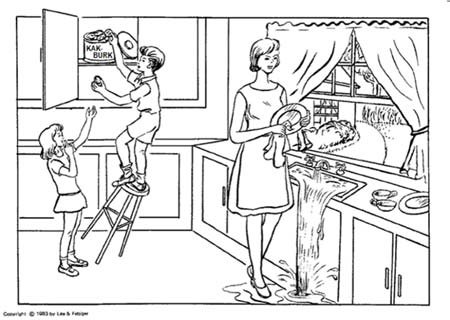
\includegraphics[width=240px, height=150px]{images/BCTPicture.png}
\caption{Cookie Theft Picture - From Kaplan and Goodglass (1983)}
\end{figure}
\par
The picture description task does a fine job of eliciting descriptive language however because of the specific content the language produce could be considered quite limited. There is some disagreement as to the benefits of this using this methodology. This task is reported as being useful to lexico-semantic disorders \cite{Boschi2017, Sajjadi2012} as the language being generated is primarly nouns and deixis (words to identify items and words to put those items into context). However, Ash \cite{Ash2012}felt that there was no difference in using this task vs Story Narration (described below). In explaining the differences, it is worth noting that these researchers were using differing variables and this could explain their different perspectives.
\par 
There are a number of existing corpus which use this tasks as the foundation of their data. The most well known is the Pitt Corpus of the Dementia Bank database. The participants of the corpus are mainly healthy controls, those with MCI and those with probable and/or possible AD. 
\subsection{Narrative description task}
The story narration task is designed to study a participant's ability to describe and elaborate on a story which is depicted using a series of pictures. The stories depicted are usually based on children's books or famous stories with the Cinderella being the one most typically used \cite{Fraser2014}. This task requires ordering the story in a structured and coherent framework. It also requires comprehension and understanding of the stories characters and the events depicted, as well as an awareness of a character's actions, motivations and internal reactions to given events. This task is particularly useful as the procedure reduces the demands on memory, due to the participant being able to access the picture book during the description and is therefore able rule out memory as a confounding variable for any results observed. As noted above, Ash \cite{Ash2012} felt that this task was interchangable with the Picture Description task. However, other research felt that this was a studier test of lexical and semantic abilities as well as syntactic complexity because this task requires interpretation and elaboration in additional to a simple description \cite{DeLira2011}. 
\par
Given the relative strengths of the Narrative description task vs Picture description task, there are few pieces of research that have used Machine Learning to analyse features from Narrative picture tasks \cite{Fraser2014}. This could be due to the availability of data and the absence of any meaningful sets of transcripts of participants performing this task. However, this could be an interesting direction to take research in the future to see if features generated from this task could be used to predict MCI or AD.  
\par
\subsection{Interviews}
Interviews can also be used to elicit language in a more natural way by asking questions to guide a conversation between speakers. There are three types of interviews: unstructured, structured and semi-structured. Structured interviews tend to produce very limited speech and therefore has never been used in this area \cite{Boschi2017}. Unstructured interviews are open ended and generally do not conform to any particular pattern. They use generic themes such as family or hobbies to guide the conversation. Whilst this is the most ecologically valid form of conversation and therefore language generation, it's unstructured nature means that the protocol cannot be consistent and therefore reproduced. Semi-structured interviews are therefore preferred over other forms of interview as a middle ground. The semi structured nature of these interviews means that there is some replicability but does not constrain the participant in answering questions.
\par
The analysis of interviews can be difficult to analyse as both the content can vary even between participants, although it can be argued that content should not affect the type of language being generated unless it is narrow topic or the participant is constrained in how they answer a given question. It is also difficult to measure as there are no pre-defined task goals in comparison to the other two methods. Nevertheless, this is the most naturalistic setting for looking at language production and can be used to look at the syntactic and semantic parts of language generation \cite{Sajjadi2012}. There have been some attempts to use interviews to assess language production in AD with promising results \cite{Asgari2017, Guinn2015}.
\par
\subsection{Conclusions}
One can view the different types of tasks above as a continuum where picture tasks represent a much more controllable task with a lot of supporting research but which generates a much more constrained set of language that is atypical of normal speech in terms of the cognitive functions used. 


\subsection{What are the goals of the studies that employ ML or Statistical Learning techniques for diagnosis of MCI or AD?}

\subsection{Do the studies focus on a one point in time or looking at cognitive deterioration over time?}

\section{Discussion and conclusions}\label{discussion}
\subsection{Discussion of the current evidence}
One of the criticisms of traditional learning models is it's reliance on features that are generated for them. As we can see from the brief look at some of the research in this field, researchers have taken a number of different approaches with success. However, there does not seem to be a consensus. As machine learning in general moves away from traditional machine learning models to deep learning techniques, it poses the question can deep learning assist with this problem?
\par 
One of the main benefits of deep learning is that it does not rely on pre defined features being fed to the model. Instead, deep learning models take raw data in with some amount of preprocessing and generates it's own features. This move away from relying on features solves one of the difficulties we have with the current psychological literature, namely that there are some disagreement on the which 
\par 
One of the drawbacks of attempting to use natural language processing and machine learning in this context is the lack of data. This is the case with all machine learning techniques, but more so with deep learning. There have been ways to 'create' more data such as data augmentation. 

Current state-of-the-art diagnostic measures of AD are invasive (CSF analysis), expensive (neuroimaging), and time-consuming (neuropsychological assessment). Furthermore, these measures are limited to speciality clinics and thus have limited accessibility as frontline screening and diagnostic tools for AD. More importantly, nonspecialists are often inaccurate at identifying early AD and MCI. Thus, there is an increasing need for additional noninvasive and/or cost-effective tools, allowing effective frontline identification of subjects in the preclinical or early clinical stages of AD who could be suitable for monitoring in speciality clinics and for early treatment. Implementation of effective screening instruments will allow diagnosis earlier in the course of dementia, even at the point when memory function is still essentially within the normal range. This strategy would enable an earlier, and potentially more effective, prevention and treatment of AD with a special focus to preserve cognitive functions.
\par 
However the literature has identified a number of challenges when approaching this problem. Firstly, the clinical features that combine to meet the diagnostic criteria for Dementia or it's variants are continuous in nature and heterogenous between patients and are also impacted by other variables. For example as shown above, cognitive performance is affected in part by a patients educational attainment and a patients ability to live independently is impacted by a their physical health as much as their cognitive health. The challenge therefore is to find features that are minimally impacted by other factors, or that can be controlled for by a experimental design such as a matched pairs design to control for educational attainment.
\par 
Another challenge lies with the recruitment of suitable individuals who may notice a decline in cognition to the point where we might classify them as having MCI, but these individuals deduce that there is little to no value to admitting there is a problem and seeking help whilst their symptoms are 'manageable'.
\par
Finally there is a large amount of variability in the presentations of those with MCI and early dementia, and this is compounded by an similar amount of variability in the criteria researchers have used for experimental groups and the approaches researchers have used to tackle this problem. This had led to a confused literature. Recently a call for research that has consistent inclusion / exclusion criteria has been made along with some proposed definitions of MCI and it's subgroups \cite{Petersen2014}. Researchers have identified the analysis of language impairment as an area of promise to explore in the diagnosis of MCI and early AD and recent developments in natural language processing and machine learning techniques have the potential to assist in this research. Indeed, given the increased burden on the diagnosis of MCI and AD on professionals there has been a call to use technology to potentially ease this burden \cite{Boschi2017}. A small but growing amount of research has gone into the use of machine learning techniques to potentially look at the automated classification of participants with MCI and/or AD, however this is a new area of research and there are some gaps in our knowledge.

\subsection{Methodological Issues}
\subsection{Limitations}

\subsection{The future of the field}
One of the main patterns 

One-class classification is a traditional machine learning model in which the object is to recognize instances of a concept by only using examples of the same concept. In the training of this model, instances of only a single object class are available during training. In this context,all other classes (any instances that deviate from the single object class) are referred to as 'alien' classes. During the testing of the model, it may encounter alien classes and the job of the model is to distinguish between objects of the known class from objects belonging to any 'alien' classes. This approach to classification has broad applications and is mainly used when there is a high cost of obtaining samples of alien classes.
\par 
In this context, we can see from 

One of the areas for research to study is a careful examination of the features that are being used to measure language deterioration. For example, Zimmerer (2016) \cite{Zimmerer2016} describes connectivity in such as a way that correlates directly with what Mueller (2018) \cite{Mueller2018a} calls Fluency. Whilst these are very nuanced measures which differ slightly in the form they take, the sheer range of measures and features being produced make it difficult to organise and explore what is truly going on in those with MCI and early AD.. Some work needs to be done in producing a consistent list of measures that are validated using existing datasets and can be used for future research moving forward. \newline
\par
Teng et al suggests that work should focus on the MCI population and concentrate on developing a consensus neuropsychological battery that could yield predictable rates of progression to AD \cite{Teng2009}. This, in conjunction with the development of a model of language, sensitive enough to detect subtle deterioration in language use to act as an additional cognitive marker to aid diagnosis could potentially move some way to providing this.
\par 
Future research should also be directed towards developing non-intrusive ways of detecting subtle changes in natural language such that any perceived deterioration that could indicate the presence of MCI or AD could be flagged up early. Machine learning approaches seem to be the most logical approach for achieving this aim as language could be collected in non-intrusive ways and passed to a machine learning algorithm for preliminary classification.  Despite the excellent quality of datasets, for example the DementiaBank dataset, being used to 'backtest' these algorithms, further research should look at generating additional datasets to increase the validity of the results found so far as well as using other methods to generate data other than Picture Description tasks which some researchers could claim are limited in scope. Finally, the recent resurgence in the use of neural networks and deep learning could provide the answer to the confused literature in terms of features. A key benefit of deep learning is it's ability to automate the process of feature engineering. So there is an opportunity to explore the use of deep learning, to not only develop new features but also validate existing features independently.  
\par
This area of research is extremely promising in its early results and the impact of successful research would be life changing for both individuals and the health of the worlds aging population in general.



\section{Conclusions}\label{conclusions}
We can see that both Natural Language Processing and Machine Learning techniques have a lot to offer, Indeed there has been a lot of research which have used pre-existing datasets to explore this area with promising results. One of the difficulties with the current research is the approach of trying to discriminate between those AD and healthy controls. This is not necessarily a problem in the real world as it is trivially easy to do for trained clinicians. A more interesting, but potentially harder to problem to solve is to discriminate between those with MCI and healthy controls, and more importantly to track their decline over time. Further, to date the authors are unaware of any research in which these techniques are applied to newly created samples of language. 


\bibliographystyle{unsrt}
\bibliography{main}

\appendix
\section{Article Table}
\begin{longtable}{ p{1cm} | p{6cm} | p{6cm}}
	\hline
	Paper Number & Paper Title & Authors \\ \hline
	1 & A Comparison of Syntax, Semantics, and Pragmatics in Spoken Language among Residents with Alzheimer's Disease in Managed-Care Facilities & C. Guinn, B. Singer, A. Habash \\ \hline
	2 & Aided Diagnosis of Dementia Type through Computer-Based Analysis of Spontaneous Speech & W. Jarrold, B. Peintner, D. Wilkins, D. Vergryi, C. Richey, M.L. Gorno-Tempini, J. Ogar \\ \hline
	3 & Automatic detection and rating of dementia of alzheimer type through lexical analysis of spontaneous speech & C. Thomas, V. Keselj, N. Cercone, K. Rockwood, E. Asp \\ \hline
	4 & Changes in Style in Authors with Alzheimer’s Disease & G. Hurst, V.W. Feng \\ \hline
	5 & Computer-based evaluation of Alzheimer's disease and mild cognitive impairment patients during a picture description task & L. Hernandez-Dominguez, S. Ratte, G. Sierra-Martinez, A. Roche-Bergua \\ \hline
	6 & Computerized neuropsychological assessment in mild cognitive impairment based on natural language processing-oriented feature extraction & C. Fang, P. Janwattanapong, H. Martin, M. Cabrerizo, A. Barreto, D. Loewenstein, R. Duara, M. Adjouadi \\ \hline
	7 & Deep-Deep Neural Network Language Models for Predicting Mild Cognitive Impairment & S.O. Orimaye, J. S-M. Wong, J. S. G. Fernandez \\ \hline
	8 & Deep language space neural network for classifying mild cognitive impairment and Alzheimer-type dementia & S.O. Orimaye, J. S-M. Wong, C.P. Wong \\ \hline 
	9 & Diagnosing people with dementia using automatic Conversation Analysis & B. Mirheidari, D. Blackburn, M. Reuber, T. Walker, H. Christensen \\ \hline
	10 & Enriching Complex Networks withWord Embeddings for Detecting Mild Cognitive Impairment from Speech Transcripts & L. B. dos Santos, E. A. Correa Jr, O. N. Oliveira Jr, D.R. Amancio, L. L. Mansur, S. M. Alusio \\ \hline
	11 & Features and Machine Learning Classification of Connected Speech Samples from Patients with Autopsy Proven Alzheimer’s Disease with and without Additional Vascular Pathology & V. Rentoumi, L. Raoufian, S. Ahmed, C. A. de Jager, P. Garrard \\ \hline
	12 & Language Analysis of Speakers with Dementia of the Alzheimer’s Type & C. Guinn, A. Habash \\ \hline
	13 & Learning Linguistic Biomarkers for Predicting Mild Cognitive Impairment using Compound Skip-grams & S. O. Orimaye, J. S-M. Wong, K. Y. Tai, C. P. Wong \\ \hline
	14 & Learning Predictive Linguistic Features for Alzheimer’s Disease and related Dementias using Verbal Utterances & S.O. Orimaye, J. S-M. Wong, K. J. Golden \\ \hline
	15 & Linguistic Features Identify Alzheimer's Disease in Narrative Speech & K. C. Fraser, J. A. Meltzer, F. Rudzicz \\ \hline
	16 & Longitudinal detection of dementia through lexical and syntactic changes in writing: a case study of three British novelists & X. Le, I. Lancashire, G. Hirst, R. Jokel \\ \hline
	17 & Multilingual word embeddings for the assessment of narrative speech in mild cognitive impairment &  K. C. Fraser, K. L. Fors, D. Kokkinakis \\ \hline
	18 & Predicting mild cognitive impairment from spontaneous spoken utterances & M. Asgari, J. Kaye, H. Dodge \\ \hline
	19 & Predicting probable Alzheimer's disease using linguistic deficits and biomarkers & S. O. Orimaye, J. S-M. Wong, K. J. Golden, C. P. Wong, I. N. Soyiri \\ \hline
	20 & Sentence segmentation in narrative transcripts from neuropsychological tests using recurrent convolutional neural networks & M. V. Treviso, C. Shulby, S. M. Alusio \\ \hline
	21 & Social Markers of Mild Cognitive Impairment: Proportion of Word Counts in Free Conversational Speech & H. H. Dodge, N. Mattek, M. Gregor, M. Bowman, A. Seelye, O. Ybarra, M. Asgari, J. A. Kaye \\ \hline
	22 & Spoken language biomarkers for detecting cognitive impairment & T. Alhanai, R. Au, J. Glass \\ \hline
	23 & Spoken Language Derivied Measures for Detecting Mild Cognitive Impairment & B. Roark, M. Mitchell, J-P. Hosom, K. Hollingshead, J. A. Kaye \\ \hline
	24 & Talk2Me: Automated linguistic data collection for personal assessment & M. Komeili, C. Pou-Prom, D. Liaqat, K. C. Fraser, M. Yancheva, F. Rudzicz \\ \hline
	25 & The Effect of Heterogeneous Data for Alzheimer’s Disease Detection from Speech & A. Balagopalan, J. Novikova, F. Rudzicz, M. Ghassemi \\ \hline
	26 & Toward the Automation of Diagnostic Conversation Analysis in Patients with Memory Complaints & B. Mirheidari, D. Blackburn, K. Harkness, T. Walker, A. Venneri, M. Reuber, H. Cristensen \\ \hline
	27 & Tracking Discourse Complexity Preceding Alzheimer's Disease Diagnosis: A Case Study Comparing the Press Conferences of Presidents Ronald Reagan and George Herbert Walker Bush & V. Berisha, S. Wang, A. LaCross, J. Liss \\ \hline
	28 & Vector-space topic models for detecting Alzheimer's disease & M. Yancheva, F. Rudzicz \\ \hline
\end{longtable}
\end{document}

%\begin{table}
%	\begin{tabular}{ p{12cm} }
%	\hline
%	(dementia OR MCI OR Mild Cognitive Impairment OR Alzheimer's OR Mild Neurocognitive Disorder OR AD) AND TOPIC: (machine learning OR Data Mining OR Decision Support System OR NLP OR Natural 			Language Processing) AND TOPIC: (prognosis OR prognostic estimate OR predictor OR prediction OR model OR patterns OR diagnosis OR diagnostic OR forecasting OR projection OR Deep Language Model 		OR Deep Neural Network) AND TOPIC: (classification OR regression OR kernel OR support vector machines OR Gaussian Process OR Bayesian Network OR Factor Analysis OR Deep Learning OR Neural 			Networks OR Maximum Likelihood OR Principal Component Analysis OR Markov OR Linear Model OR Mixture Model OR Perceptron Algorithm OR Logical Learning OR relational learning OR Supervised 				Learning OR Unsupervised Learning OR clustering OR Decision Tree) AND TOPIC: (Language OR Cognitive OR Speech OR Conversation OR Connected Speech OR Picture Description OR Discourse Analysis OR 		Verbal Fluency)  \\ \hline
%	Searched - 4th April 2019 - Generated 1257 Articles \\
%	\hline
%	\end{tabular}
%	\caption[Table caption text]{Search Terms for Scopus database}
%	\label{table:name}
%\end{table}
%
%\begin{table}
%	\begin{tabular}{ p{12cm} }
%	\hline
%	(dementia OR MCI OR Mild Cognitive Impairment OR Alzheimer's OR Mild Neurocognitive Disorder OR AD) AND TOPIC: (machine learning OR Data Mining OR Decision Support System OR NLP OR Natural 			Language Processing) AND TOPIC: (prognosis OR prognostic estimate OR predictor OR prediction OR model OR patterns OR diagnosis OR diagnostic OR forecasting OR projection OR Deep Language Model 		OR Deep Neural Network) AND TOPIC: (classification OR regression OR kernel OR support vector machines OR Gaussian Process OR Bayesian Network OR Factor Analysis OR Deep Learning OR Neural 			Networks OR Maximum Likelihood OR Principal Component Analysis OR Markov OR Linear Model OR Mixture Model OR Perceptron Algorithm OR Logical Learning OR relational learning OR Supervised 				Learning OR Unsupervised Learning OR clustering OR Decision Tree) AND TOPIC: (Language OR Cognitive OR Speech OR Conversation OR Connected Speech OR Picture Description OR Discourse Analysis OR 		Verbal Fluency)  \\ \hline
%	Searched - 4th April 2019 - Generated 1257 Articles \\
%	\hline
%	\end{tabular}
%	\caption[Table caption text]{Search Terms for ProQuest database}
%	\label{table:name}
%\end{table}
%
%\begin{table}
%	\begin{tabular}{ p{12cm} }
%	\hline
%	(dementia OR MCI OR Mild Cognitive Impairment OR Alzheimer's OR Mild Neurocognitive Disorder OR AD) AND TOPIC: (machine learning OR Data Mining OR Decision Support System OR NLP OR Natural 			Language Processing) AND TOPIC: (prognosis OR prognostic estimate OR predictor OR prediction OR model OR patterns OR diagnosis OR diagnostic OR forecasting OR projection OR Deep Language Model 		OR Deep Neural Network) AND TOPIC: (classification OR regression OR kernel OR support vector machines OR Gaussian Process OR Bayesian Network OR Factor Analysis OR Deep Learning OR Neural 			Networks OR Maximum Likelihood OR Principal Component Analysis OR Markov OR Linear Model OR Mixture Model OR Perceptron Algorithm OR Logical Learning OR relational learning OR Supervised 				Learning OR Unsupervised Learning OR clustering OR Decision Tree) AND TOPIC: (Language OR Cognitive OR Speech OR Conversation OR Connected Speech OR Picture Description OR Discourse Analysis OR 		Verbal Fluency)  \\ \hline
%	Searched - 4th April 2019 - Generated 1257 Articles \\
%	\hline
%	\end{tabular}
%	\caption[Table caption text]{Search Terms for IEEE Xplore database}
%	\label{table:name}
%\end{table}